\pdfoutput=1
\documentclass[twocolumn]{aastex61}
%%\documentclass[]{emulateapj}

%Accepted/received/... %%

\received{xxx}
\revised{yyy}
\accepted{zzz}

%% Command to document which AAS Journal the manuscript was submitted to.
\submitjournal{AAS Journals}

%% Short title/authors

\shorttitle{Tidal Locking in Stellar Binaries}
\shortauthors{Fleming \& Barnes}

%% Begin document, title, packages %%
\usepackage{hyperref}
\usepackage{xspace}
\usepackage{graphicx}
\usepackage{amsmath}
\usepackage[caption=false]{subfig}

%% Custom commands
\def\mearth{{\rm\,M_\oplus}}
\def\rearth{{\rm\,R_\oplus}}
\def\msun{{\rm\,M_\odot}}
\def\rsun{{\rm\,R_\odot}}
\def\lsun{{\rm\,L_\odot}}
\def\gsim{~\rlap{$>$}{\lower 1.0ex\hbox{$\sim$}}}
\def\lsim{~\rlap{$<$}{\lower 1.0ex\hbox{$\sim$}}}

\newcommand{\vplanet}[0]{\texttt{VPLanet}\xspace}
\newcommand{\eqtide}[0]{\texttt{EQTIDE}\xspace}
\newcommand{\stellar}[0]{\texttt{STELLAR}\xspace}
\newcommand{\kepler}[0]{\textit{Kepler}\xspace}


%% Begin doc %%

\begin{document}

\title{Tidal Locking in Low-Mass Stellar Binary Stars}

%% AUTHORS %%

%%\correspondingauthor{David P. Fleming}
%%\email{dflemin3@uw.edu}

%%\author[0000-0001-9293-4043]{David P. Fleming}
\author{David P. Fleming}
\affil{Astronomy Department, University of Washington \\
Box 951580, Seattle, WA 98195}

\author{Rory Barnes}
\affiliation{Astronomy Department, University of Washington \\
Box 951580, Seattle, WA 98195}

%% ABSTRACT %%

\begin{abstract}

Abstract

\end{abstract}

%% KEYWORDS %%

\keywords{binaries: close}

%% INTRO %%

\section{Introduction} \label{sec:intro}

XXX

tidal locking assumed for short period binaries, tsync << tcirc eg Mazeh 2008, so some have speculated that low-mass binaries can synchronize out to longer orbital periods.  tentative evidence for this in Lurie 2017 data, discuss pseudosyncronization, synchronization, \citet{Counselman1973} tidal end states

we give a shit about sync binaries as they are fast rotators, e.g. what \citet{Simonian2018} might be seeing in \kepler field, can have enhanced magnetic activity (short Prot -> enhanced Lxuv), impact gyrochronology predictions, it's a fundamental evolutionary process for roughly half of sun like stars.

dank plot showing average tsync for various orbital period ranges for CPL vs CTL marginalizing over all other parameters. do it with small multiples

%% SECTION : Methods %%

\section{Methods} \label{sec:methods}

\subsection{Stellar Evolution} \label{sec:methods:stellar}

XXX

We simulate stellar rotation evolution for both single stars and stellar binaries using the coupled stellar-tidal evolution model presented in \citet{Fleming2018} and implemented in the open-source code VPLanet\footnote{VPLanet is publically available
at \href{https://github.com/VirtualPlanetaryLaboratory/vplanet}{{https://github.com/VirtualPlanetaryLaboratory/vplanet}}.} \citep[][Barnes et al., in prep]{Barnes2016,vplanet2018}. We improve upon the stellar evolution model used in \citet{Fleming2018}, \stellar, by tracking the evolution of both the stellar radius of gyration, $r_g$, and radius, using a bicubic interpolation over mass and time of the \citet{Baraffe2015} stellar evolution models. We model stellar spin-down due to magnetic braking using the model derived in \citet{Matt2015} since it has been shown to successfully reproduce many features in the P$_{rot}$ distribution of the \textit{Kepler} field, notably the upper and lower envelopes of the latter distribution and the observed ``dip" in the distribution around M${\approx}0.6$ M$_{\odot}$. We integrate the following equation to model the net change in the stellar rotation rate due to stellar evolution and magnetic braking: 

\begin{equation} \label{eqn:stellar_rot_rate_dt}
\dot{\omega} = \frac{\dot{J}_{mb}}{I} - \frac{2 \dot{R} \omega}{R} - \frac{2 \dot{r_g} \omega}{r_g}
\end{equation}
where the moment of inertia $I = M r_g^2 R^2$ and $\dot{J}_{mb}$ is the angular momentum loss due to magnetic braking.  

\subsection{Tidal Evolution} \label{sec:methods:eqtide}

 Equilibrium tidal models, first introduced by \citep{Darwin1880}, track the secular evolution of an orbiter's semi-major axis, $a$, eccentricity, $e$, and the rotation rates, $\omega$, and obliquities $\psi$, of the tidally-interacting bodies subject to tidal torques. Equilibrium tidal models assume that tidally-interacting bodies raise tidal bulges on their companions that are offset from the line connecting the both bodies' centers of mass, driving torques that exchange angular momentum between the orbit and both bodies' spins. Equilibrium tidal models are linear since the tidal waves that comprise the tidal bulge on a body are assumed to be uncoupled. Under these assumptions, the tidal evolution is analogous to a driven, damped harmonic oscillator \citep{Greenberg2009}.  We refer the reader to \citet{Barnes2017} for an in-depth discussion of the assumptions and limitations of equilibrium tidal models.  Although simple, equilibrium tidal models have been used to robustly model the secular orbital and rotation evolution of both exoplanets \citet[e.g.][]{Goldreich1966,Jackson2009,Leconte2010,Heller2011,Barnes2013,Barnes2017} and stellar binaries \citep[e.g.][]{Repetto2014,Fleming2018}.  Here, we consider two equilibrium tidal models to study the secular spin-orbital evolution of low-mass stellar binaries.  

\subsubsection{Constant Phase Lag (CPL) Model}

The ``Constant Phase Lag" (CPL) \citep[][]{FerrazMello2008,Heller2011} equilibrium tidal model assumes that the tidal torque on one body due to its companion arises from a linear combination of several discrete, uncoupled tidal bulges, each with their own associated frequency, that maintain a fixed phase with respect to the line connecting the two stars' centers of mass. We use the \eqtide implementation of the CPL model in VPLanet following the derivation of \citet{FerrazMello2008}.  The equations that govern the secular change in $e$ and $a$ are as follows:

\begin{equation} \label{eqn:cpl_e}
\frac{de}{dt} = -\frac{ae}{8 G m_1 m_2} \sum_{i=1}^2 Z_{i,\mathrm{CPL}} \left( 2 \varepsilon_{0,i} - \frac{49}{2} \varepsilon_{1,i} + \frac{1}{2} \varepsilon_{2,i} + 3 \varepsilon_{5,i} \right)
\end{equation}
\begin{equation} \label{eqn:cpl_a}
\frac{da}{dt} = \sum_{i=1}^2 \frac{da_i}{dt}
\end{equation}
where if the $i^{th}$ body is tidally-locked in a synchronous orbit,
\begin{equation} \label{eqn:cpl_dadt_locked}
\frac{da_{i,sync}}{dt} = -\frac{a^2}{G m_1 m_2} Z_{i,\mathrm{CPL}} \left( 7 e^2 + \sin^2 (\psi_i) \right) \varepsilon_{2,i},
\end{equation}
otherwise
\begin{equation}
\begin{split}
\frac{da_i}{dt} & = \frac{a^2}{4 G m_1 m_2} Z_{i,\mathrm{CPL}} \left( 4 \varepsilon_{0,i} + e^2 \left[ -20 \varepsilon_{0,i} + \frac{147}{2} \varepsilon_{1,i} \right. \right. \\
&  + \left. \left. \frac{1}{2} \varepsilon_{2,i} - 3 \varepsilon_{5,i} \right] - 4 \sin^2 (\psi_i) \left[ \varepsilon_{0,i} - \varepsilon_{8,i} \right] \right).
\end{split}
\end{equation}
The CPL equations for $\psi$ and $\omega$ evolution are
\begin{equation} \label{eqn:cpl_psi}
\frac{d\psi_i}{dt} = \frac{Z_{i,\mathrm{CPL}} \sin(\psi_i)}{4 m_i r_{g,i}^2 R_i^2 n \omega_i} \left( [1-\xi_i] \varepsilon_{0,i} + [1+\xi_i](\varepsilon_{8,i} - \varepsilon_{9,i}) \right)
\end{equation}
\begin{equation} \label{eqn:cpl_omega}
\begin{split}
\frac{d\omega_i}{dt}& = -\frac{Z_{i,\mathrm{CPL}}}{8m_i r_{g,i}^2 R_i^2 n} \left(4 \varepsilon_{0,i} + e^2\left[-20\varepsilon_{0,i} + 49\varepsilon_{1,i} + \varepsilon_{2,i} \right] \right. \\
& \left. + 2 \sin^2(\psi_i) \left[ -2 \varepsilon_{0,i} + \varepsilon_{8,i} + \varepsilon_{9,i} \right] \right)
\end{split}
\end{equation}
where $G$ is Newton's gravitational constant, $n$ is the binary's mean motion, and the index $i$ denotes that $i^{th}$ body. The tidal phase lags signs, $\varepsilon$, for the $i^{th}$ body are given by
\begin{equation} \label{eqn:cpl_eps}
\begin{split}
\varepsilon_{0,i} & = \Sigma(2 \omega_i - 2n) \\
\varepsilon_{1,i} & = \Sigma(2 \omega_i - 3n) \\
\varepsilon_{2,i} & = \Sigma(2 \omega_i - n) \\
\varepsilon_{5,i} & = \Sigma(n) \\
\varepsilon_{8,i} & = \Sigma(\omega_i - 2n) \\
\varepsilon_{9,i} & = \Sigma(\omega_i)
\end{split}
\end{equation}
where the function $\Sigma(x)$ returns $1$ for positive $x$, $-1$ for negative $x$, and $0$ otherwise.

The intermediate variable $Z_{\mathrm{CPL},i}$ is given by
\begin{equation} \label{eqn:cpl_z}
Z_{i,\mathrm{CPL}} = 3 G^2 k_{2,i} m_j^2 (m_1 + m_2) \frac{R_i^5}{a^9} \frac{1}{n Q_i}
\end{equation}
where the $j^{th}$ body is the $i^{th}$ body's companion, $k_{2}$ is the body's Love number of degree 2, and $Q$ is the tidal quality factor (``tidal Q"). The tidal Q parameterizes the energy dissipation due to tidal evolution, with lower tidal Qs, i.e. larger phase differences between the tidal bulges, driving more rapid tidal evolution.

$\xi_i$ is defined as
\begin{equation}\label{eqn:cpl_chi}
\xi_i = \frac{r_{\mathrm{g},i}^2 R_i^2 \omega_i a n }{ G M_j}.
\end{equation}

%Following \citet{Fleming2018}, when one or both binary stars are tidally locked, we assume that tidal forces prevent magnetic braking from spinning down the tidally locked star(s), but instead, any angular momentum lost is lost at the expense of the binary orbit, decreasing the orbital semi-major axis as a result.  Below in Eq.~(\ref{eqn:tidal_locked_one}) and Eq.~(\ref{eqn:tidal_locked_two}), we modify Eqs. (18) and (20) from \citet{Fleming2018} to account for $r_g$ evolution for the cases when one or both stars tidally lock under conservation of angular momentum, respectively:
%\small
%\begin{equation} \label{eqn:tidal_locked_one}
%\begin{split}
%\dot{a}_{coupled}^{(1)} = \frac{-\dot{J_{mb}} - 2 \omega \left( m_1 r_{g,1}^2 R_1 \dot{R_1} - m_1 r_{g,1} \dot{r}_{g,1} R_1^2 \right)}
%{\frac{\mu^2 G M (1-e^2)}{2J_{orb}} - \frac{3 \omega}{2a} m_1 r_{g,1}^2 R_1^2}
%\end{split}
%\end{equation}
%\normalsize
% and
% \small
%\begin{equation} \label{eqn:tidal_locked_two}
%\begin{split}
%\dot{a}_{coupled}^{(2)} = \frac{-\dot{J_{mb}} - 2 \omega \left( \sum_{i=1}^{2} m_i r_{g,i}^2 R_i \dot{R_i} + m_i r_{g,i} \dot{r}_{g,i} R_i^2 \right)}
%{\frac{\mu^2 G M (1-e^2)}{2J_{orb}} - \frac{3 \omega}{2a} \left( m_1 r_{g,1}^2 R_1^2 + m_2 r_{g,2}^2 R_2^2 \right)}
%\end{split}
%\end{equation}
%\normalsize
%where $J_{orb}$ is the orbital angular momentum.

\subsubsection{Constant Time Lag (CTL) Model}

The ``Constant Time Lag" (CTL) \citep[][]{Hut1981,Leconte2010} equilibrium tidal model assumes a constant time interval between the body's tidal bulge and the passage of the tidally-interacting companion. In this formalism, unlike the CPL model, the CTL model is continuous over a range of tidal wave frequencies.  However if the assumption of linearity is relaxed, i.e. frequencies associate with tidal bulges are allowed to depend on a spin or orbital forcing frequency, then this model is only valid over a small range of frequencies \citep{Greenberg2009}. We use the \eqtide implementation of the CTL model in VPLanet following the derivation of \citet{Leconte2010}.  The equations that govern the secular change in $e$, $a$, $\omega$, and $\psi$ are as follows:

\begin{equation} \label{eqn:ctl_e}
  \frac{de}{dt} = \frac{11 ae}{2 G M_1 M_2}
  \sum_{i = 1}^2 Z_{\mathrm{CTL},i} \left( \cos(\psi_i) \frac{f_4(e)}{\beta^{10}(e)}  \frac{\omega_i}{n} -\frac{18}{11} \frac{f_3(e)}{\beta^{13}(e)}\right),
\end{equation}

\begin{equation}\label{eqn:ctl_a}
  \frac{da}{dt} \ = \  \frac{2 a^2}{G M_1 M_2}
  \sum\limits_{i = 1}^2 Z_{\mathrm{CTL},i} \left( \cos(\psi_i) \frac{f_2(e)}{\beta^{12}(e)} \frac{\omega_i}{n} - \frac{f_1(e)}{\beta^{15}(e)}\right),
\end{equation}

\begin{equation}\label{eqn:ctl_o}
  \frac{d\omega_i}{dt} \ = \ \frac{Z_{\mathrm{CTL},i}}{2 M_i r_{g,i}^2 
R_i^2 n} \left( 2 \cos(\psi_i) \frac{f_2(e)}{\beta^{12}(e)} - \left[ 1+\cos^2(\psi)
 \right] \frac{f_5(e)}{\beta^9(e)} 
\frac{\omega_i}{n} \right),  
\end{equation}
and
\begin{equation}\label{eqn:ctl_psi}
  \frac{d\psi_i}{dt} = \frac{Z_{\mathrm{CTL},i} \sin(\psi_i)}{2 M_i r_{g,i}^2 R_i^2 n \omega_i}\left( \left[ \cos(\psi_i) - \frac{\xi_i}{ \beta} \right] \frac{f_5(e)}{\beta^9(e)} \frac{\omega_i}{n} - 2 \frac{f_2(e)}{\beta^{12}(e)} \right).
\end{equation}
where the intermediate variables are given by 
\begin{equation}\label{eqn:ctl_z}
 Z_{i,\mathrm{CTL}} = 3 G^2 k_{2,i} M_j^2 (M_i+M_j) \frac{R_i^5}{a^9} \tau_i ,
\end{equation}
and 
\begin{equation}\label{eqn:ctl_f_e}
\begin{array}{l}
\beta(e) = \sqrt{1-e^2},\\
f_1(e) = 1 + \frac{31}{2} e^2 + \frac{255}{8} e^4 + \frac{185}{16} e^6 + \frac{25}{
64} e^8,\\
f_2(e) = 1 + \frac{15}{2} e^2 + \frac{45}{8} e^4 + \frac{5}{16} e^6,\\
f_3(e) = 1 + \frac{15}{4} e^2 + \frac{15}{8} e^4 + \frac{5}{64} e^6,\\
f_4(e) = 1 + \frac{3}{2} e^2 + \frac{1}{8} e^4,\\
f_5(e) = 1 + 3 e^2 + \frac{3}{8} e^4.
\end{array}
\end{equation}

In both the CPL and CTL model, We assume $k_2 = 0.5$. This choice of $k_2$ does not impact our results as $k_2$ is degenerate with Q in the CPL model, e.g. the $k_2/Q$ scaling in Eq.~(\ref{eqn:cpl_z}), and with $\tau$ in the CTL model, e.g. $k_2 \tau$ scaling in Eq.~(\ref{eqn:ctl_z}), so we instead examine how our results scale with $Q$ and $\tau$.

\subsubsection{Tidal Locking and Numerical Integration}

XXX discuss integration specifics, equilbrium rotation rates, timestepping, $4^{th}$ order Runge-Kutta scheme.

\subsubsection{Example Tidal Evolution}

Here in Fig.~\ref{fig:tidalExample} we plot the example tidal evolution for $a$, $e$, and $\omega$, ignoring stellar evolution, for a solar-twin binary with an initial P$_{orb} = 10$ d, P$_{rot} = 1$ d, $e = 0.2$ for the CPL model and CTL model, assuming $Q=10^6$ and $\tau = 0.1$ seconds, respectively.

\begin{figure}[h]
	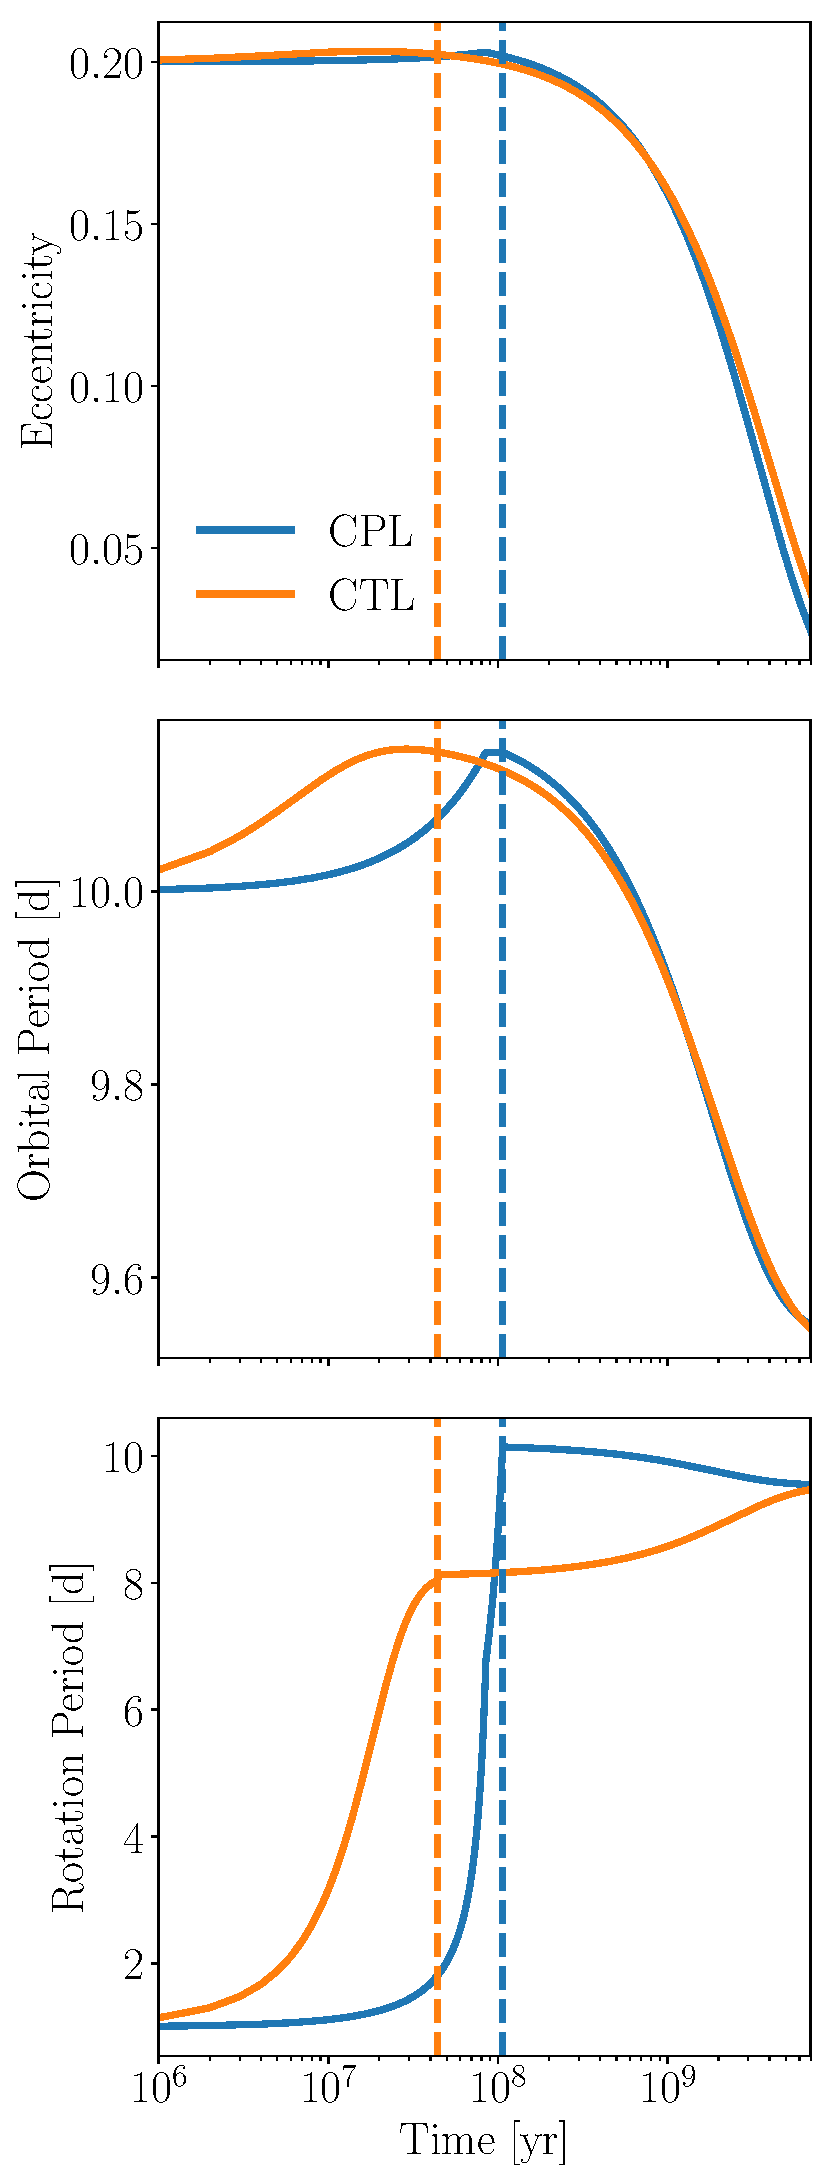
\includegraphics[width=\columnwidth]{../Plots/tidalExample.pdf}
   \caption{Spin-orbital tidal evolution of a 1 M$_{\odot} -$ 1 M$_{\odot}$ stellar binary. XXX}%
    \label{fig:tidalExample}%
\end{figure}

%% SECTION: Simulations + Initial conditions %%

\section{Simulations} \label{sec:simulations}

XXX

- we consider eccentricities up to 0.3 as the CPL model fails above that.  CTL model can handle it, but at high eccentricity, dynamical tide, e.g. dissipation via waves and stuff, becomes important

%% SECTION: VPLANET RESULTS %%

\section{Results} \label{sec:results}

XXX

%\begin{figure*}[ht]
%	\includegraphics[width=\textwidth]{../Plots/kepler_two_pop_box_dist.pdf}
%   \caption{Identical format to Fig.~\ref{fig:kepler1}, but displaying simulated data from our two population model (see $\S$~\ref{sec:results:kepler_two_pop}). Our two population model reproduces the observed \textit{Kepler} P$_{rot}$ distribution, especially the fast rotator population, with a total median P$_{rot} = 19.6$ d compared to the \textit{Kepler} median P$_{rot} = 17.3$ d, a close match. In the right panel for $ 0.4 \textrm{M}_{\odot} \lsim \textrm{M} \lsim 1.2 \textrm{M}_{\odot}$, the inclusion of tidally-interacting binaries in the total (blue) sample leads to an excellent match with the \textit{Kepler} distribution (red) compared to the single-star only (orange) model, emphasizing the importance of including stellar binaries in P$_{rot}$ forward models.}%
%    \label{fig:kepler_two_pop}%
%\end{figure*}

%% SECTION: DISCUSSION %%

\section{Discussion} \label{sec:discussion}

XXX

%% ACKNOWLEDGEMENTS %%
\acknowledgments
This work was facilitated though the use of advanced computational, storage, and networking infrastructure provided by the Hyak supercomputer system and funded by the STF at the University of Washington. This work was supported by NASA Headquarters under the NASA Earth and Space Science Fellowship Program - Grant 80NSSC17K0482.  DPF and RB acknowledge that this work was supported by the NASA Astrobiology Institute's Virtual Planetary Laboratory under Cooperative Agreement number NNA13AA93A. 

%% SOFTWARE %%
%\software{matplotlib: \citet{Hunter2007}, numpy: \citet{vanderWalt2011}, pandas: \citet{Mckinney2010}}

%% BIBLIOGRAPHY %%
\bibliography{sync}

\end{document}

%% End document %%
